There is a possibility to deploy an agent application on machines with different resource profiles and therefore it is important to determine how algorithms are performing given different resource limits.
In this test 4 agent profiles with limited CPU and memory were considered:
\begin{table}[H]
\centering
\begin{tabular}{@{}lll@{}}
\toprule
Profile name     & Memory limit & CPU limit \\ \midrule
very low profile & 128 MB        & 0.1 CPU   \\
low profile      & 128 MB        & 0.2 CPU   \\
medium profile   & 256 MB        & 0.3 CPU   \\
high profile     & 800 MB        & 1.0 CPU     \\ \bottomrule
\end{tabular}%
\end{table}

Memory limit refers to the maximum amount of memory that can be used before the process running application in the agent will be terminated. CPU limit will ensure that the agent can only use a specific part of the host CPU resources, i.e. setting it to 0.5 will produce the same output as running an application with 2 times slower CPU\cite{docker_container_limits}. A time limit of 10s was given to the agents while performing computations.

A comparison of agents running with different resource profiles according to the percentage of paths found can be seen in figure \ref{fig:compare_profiles_paths}. In the case of the first free algorithms(A*, Cloud A*, Cloud CA*), agents are able to find all possible paths which are equal to around 95\% of the total number of paths for all resources profile. 

In the case of the CA* algorithm, agents with very low profiles can only find 50\% of the total path given, low profile 65\%, medium profile - nearly 80\%, and high profile 95\%. 
\begin{figure}[H]
    \centering
    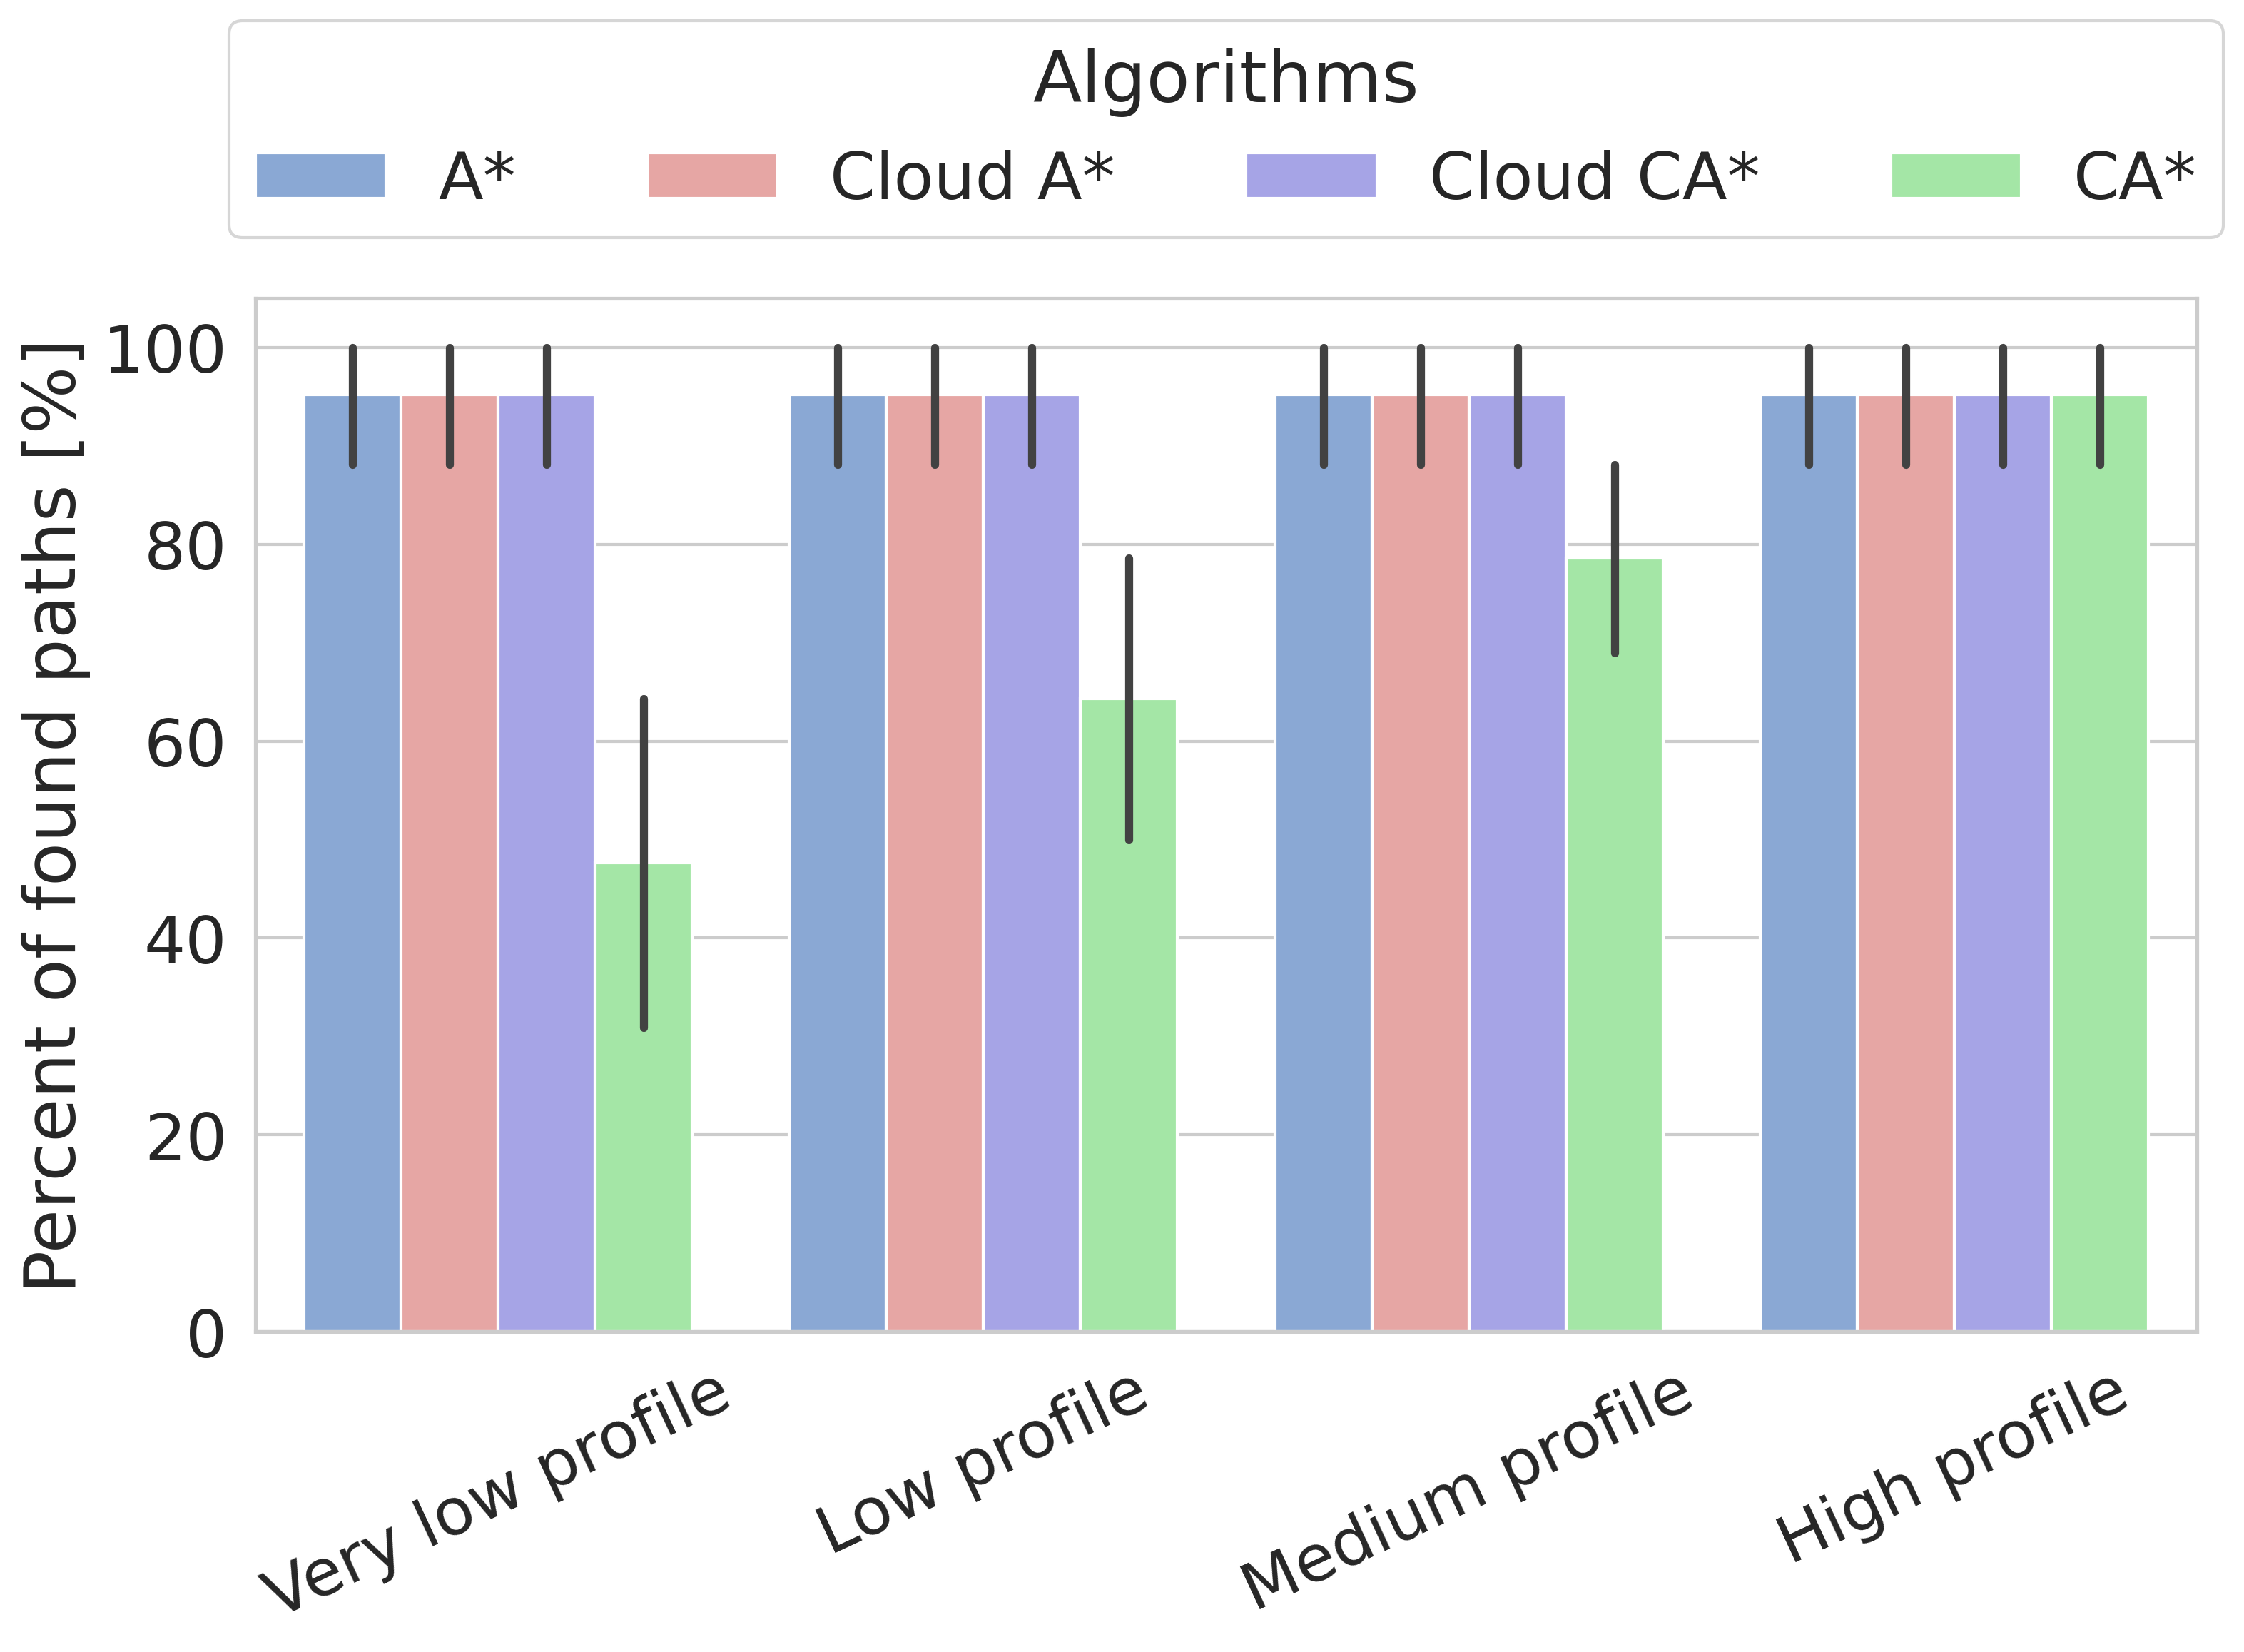
\includegraphics[width=0.8\textwidth]{pictures/compare_profiles_paths.png}
    \caption{Percentage of paths found by an agent with different resources profile
    }
    \label{fig:compare_profiles_paths}
\end{figure}

Figure \ref{fig:compare_profiles_log} shows the performance of agents with different resource profiles in relation to the average computing time for all agents. Time is given in milliseconds and shown on a logarithmic scale.

An agent with the low resource profile performed similarly for A* and cloud A* algorithms, however, Cloud CA* computing time was more than 10x smaller than local CA*. Further increase of agent resources, results in lowering of computing time. For agents with high resources, A* performed significantly better than cloud A*, and results from cloud CA* and CA* were similar, but cloud CA* performed better.
\begin{figure}[H]
    \centering
    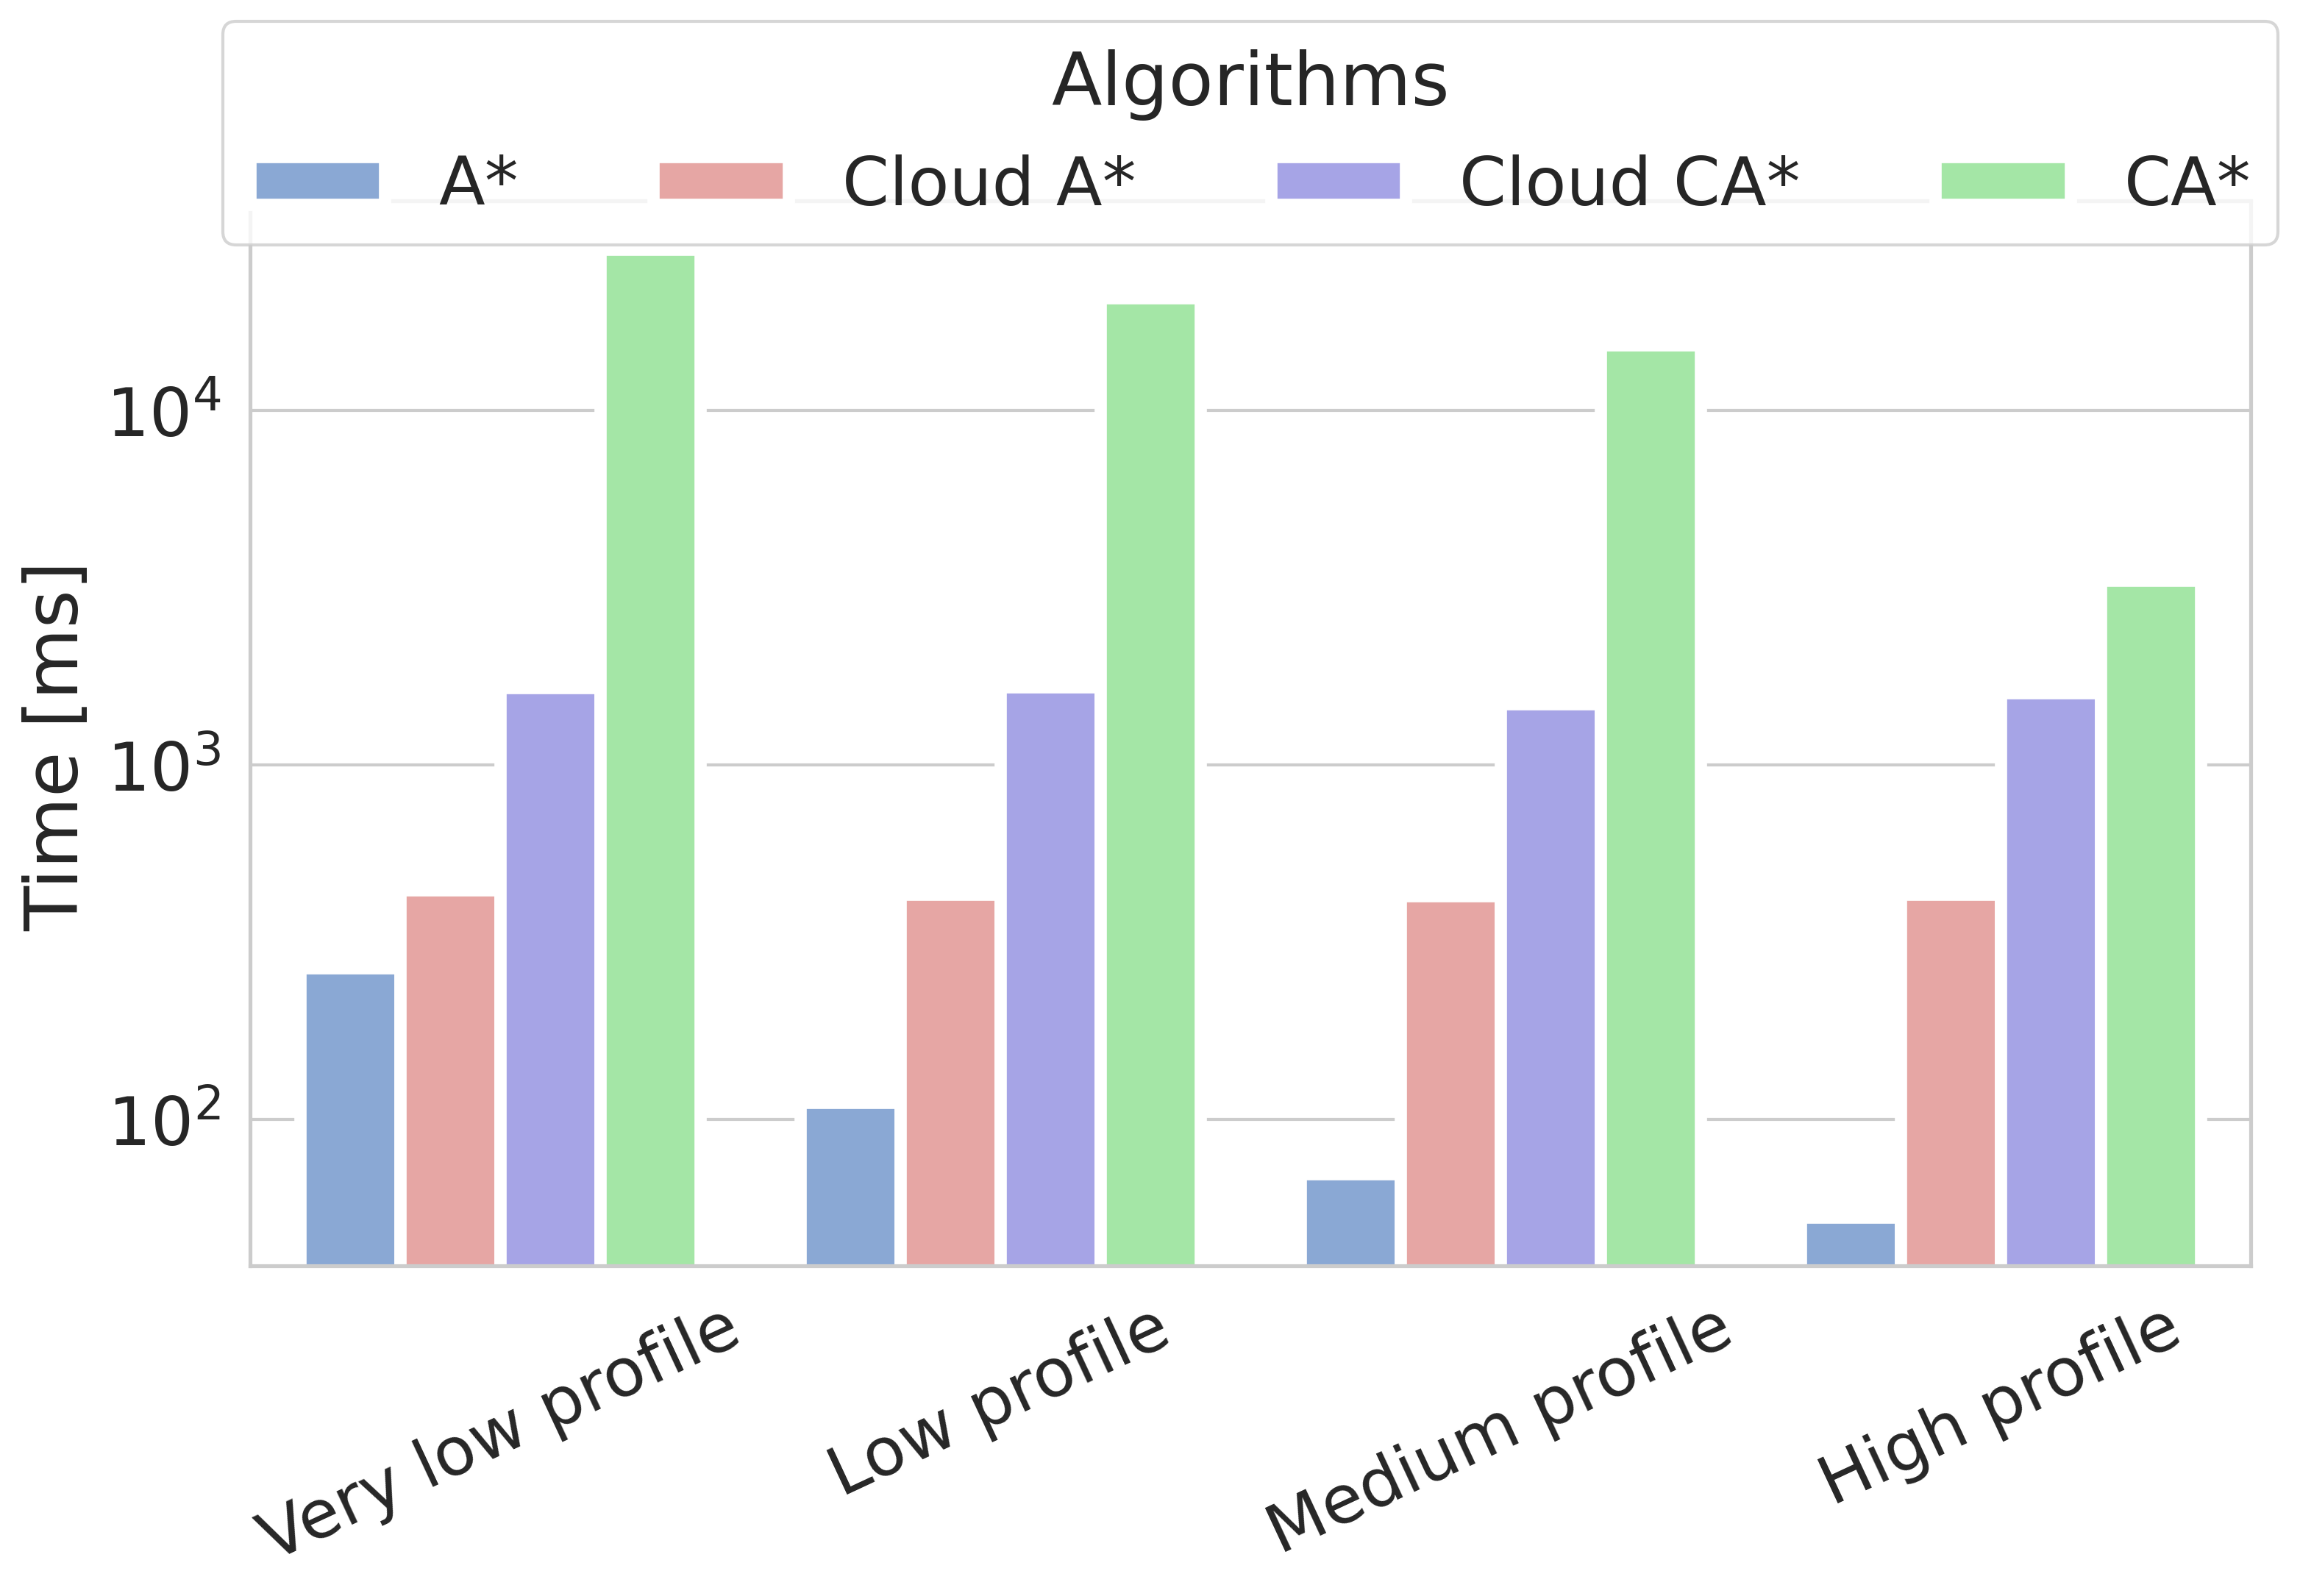
\includegraphics[width=0.8\textwidth]{pictures/compare_profiles_log.png}
    \caption{Difference in compute time by agent resources}
    \label{fig:compare_profiles_log}
\end{figure}